\documentclass{article}

\usepackage{url}
\usepackage{amsmath,amssymb}
\usepackage{graphicx}

\begin{document}
\title{Lecture N\\ The Title}
\author{C.L. Wyatt}
\date{\today}
\maketitle

In today's lecture we learn some stuff.

\begin{itemize}
\item thing one
\item thing two
\end{itemize}

\section{Introduction Section}

Here is a figure to look at.

\begin{figure}
  \centering
  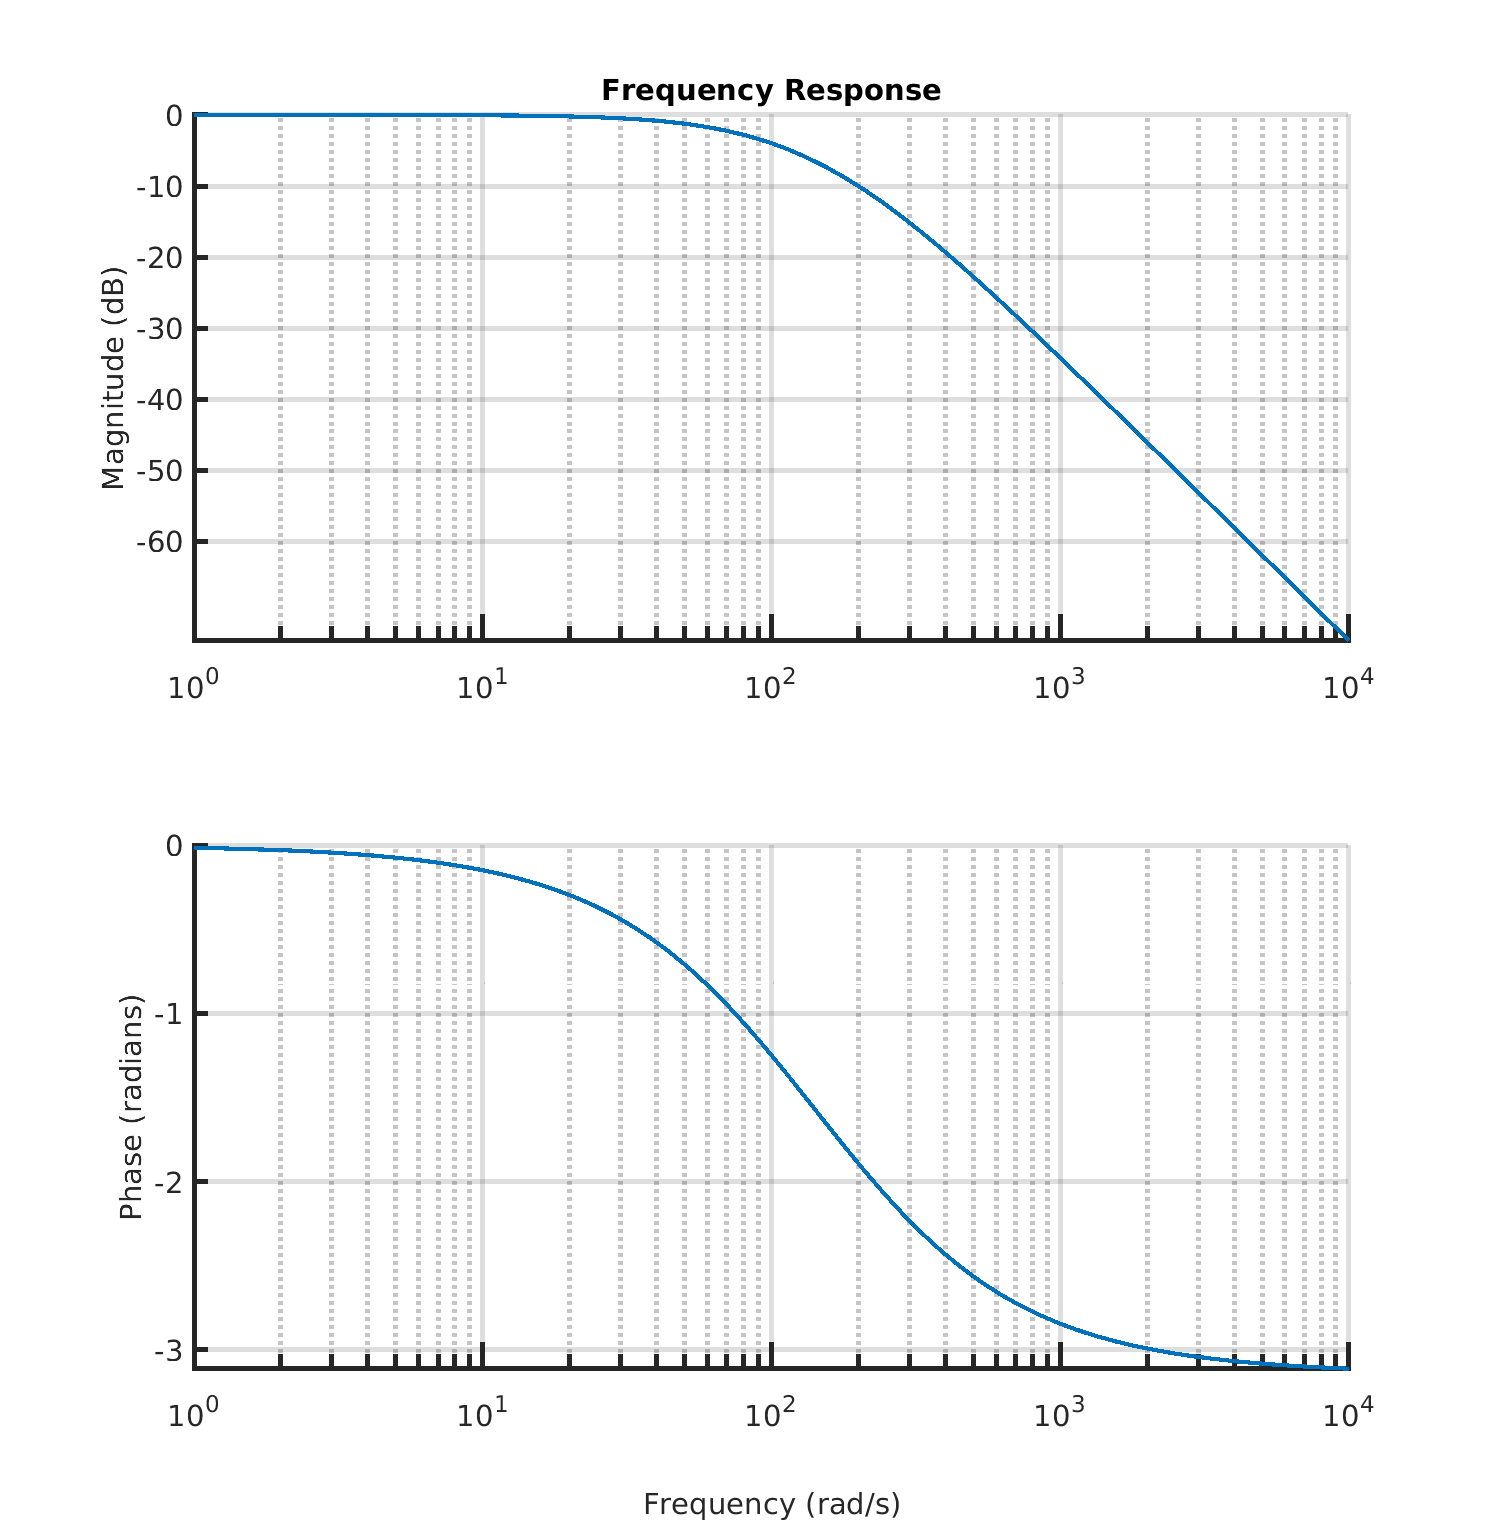
\includegraphics[alt={Description Here}]{lecture20_1.png}
  \caption{The Caption}
\end{figure}

Here is a table:

\begin{table}
  \centering
  \begin{tabular}{ccc}
    A & B & C\\\hline
    D & E & F\\
    G & H & $x^2$\\
    \hline
  \end{tabular}
\end{table}


The following is a section with some math.

\section{Convolution Integral}

To derive this we start with the sifting property of the CT impulse function (from chapter 2)
\[
\int\limits_{a}^{b} x(t)\delta(t-t_0) \; dt = x(t_0)
\]
for any $a < t_0 < b$. A slight change of variables ($t_0 \rightarrow \tau$) and limits ($a \rightarrow -\infty$ and $b \rightarrow \infty$) gives:
\[
x(t) = \int\limits_{-\infty}^{\infty} x(\tau)\delta(t-\tau) \; d\tau
\]
showing that we can write any CT signal as an infinite sum (integral) of weighted and time-shifted impluse functions.

Let $h(t)$ be the CT {\it impulse response}, the output due to the input $\delta(t)$, i.e. $\delta(t) \mapsto h(t)$. Then if the system is time-invariant: $\delta(t-\tau) \mapsto h(t-\tau)$ and by superposition if the input is writen as
\[
x(t) = \int\limits_{-\infty}^{\infty} x(\tau)\delta(t-\tau) \; d\tau
\]
then the output is given by
\[
  y(t) = \int\limits_{-\infty}^{\infty} x(\tau)h(t-\tau) \; d\tau = x(t) * h(t)
\]
This is called the \emph{convolution integral} \index{CT Convolution}.

It is worth pausing here to see the signifigance. For a LTI CT system, if I know its impulse response $h(t)$, I can find the response due to \textbf{any} input using convolution. For this reason the impulse response is another way to represent an LTI system.

\end{document}
